\section{Diskussion}
\label{sec:Diskussion}
Die Messung der Stabilitätsbedingung verlief ohne Probleme und konnte die theoretischen
Überlegungen zur Stabilität des Laserstrahls bestätigen.
Auch die Intensitätsverteilung der TEM Moden entspricht der Erwartung, was die gute
Übereinstimmung der Messwerte mit dem Fit der Theoriekurve nachweist.

Die Betrachtung der Frequenzbreite konnte den Multimodenbetrieb des Laser eindeutig begründen.
Alle berechneten Resonaterlängen stimmen sehr gut mit dem tatsächlich eingestellten Längen überein.

Mithilfe der Beugungsmuster wurde der Mittelwert der Wellenlänge zu $\lambda =\qty{639+-5}{\nano\metre}$
bestimmt. Dieser ist unter Berücksichtigung des Fehlers nahezu mit der theoretischen Wellenlänge \cite{laser} des
He-Ne Lasers von $\lambda_{\text{theorie}} =\qty{633.8}{\nano\metre}$ vereinbar.
Die geringe ABweichung stammt wahrscheinlich aus Ableseungenauigkeiten der Beugungsmaxima am Schirm.

\section{Anhang}
\label{sec:Anhang}
\begin{figure}
    \centering
    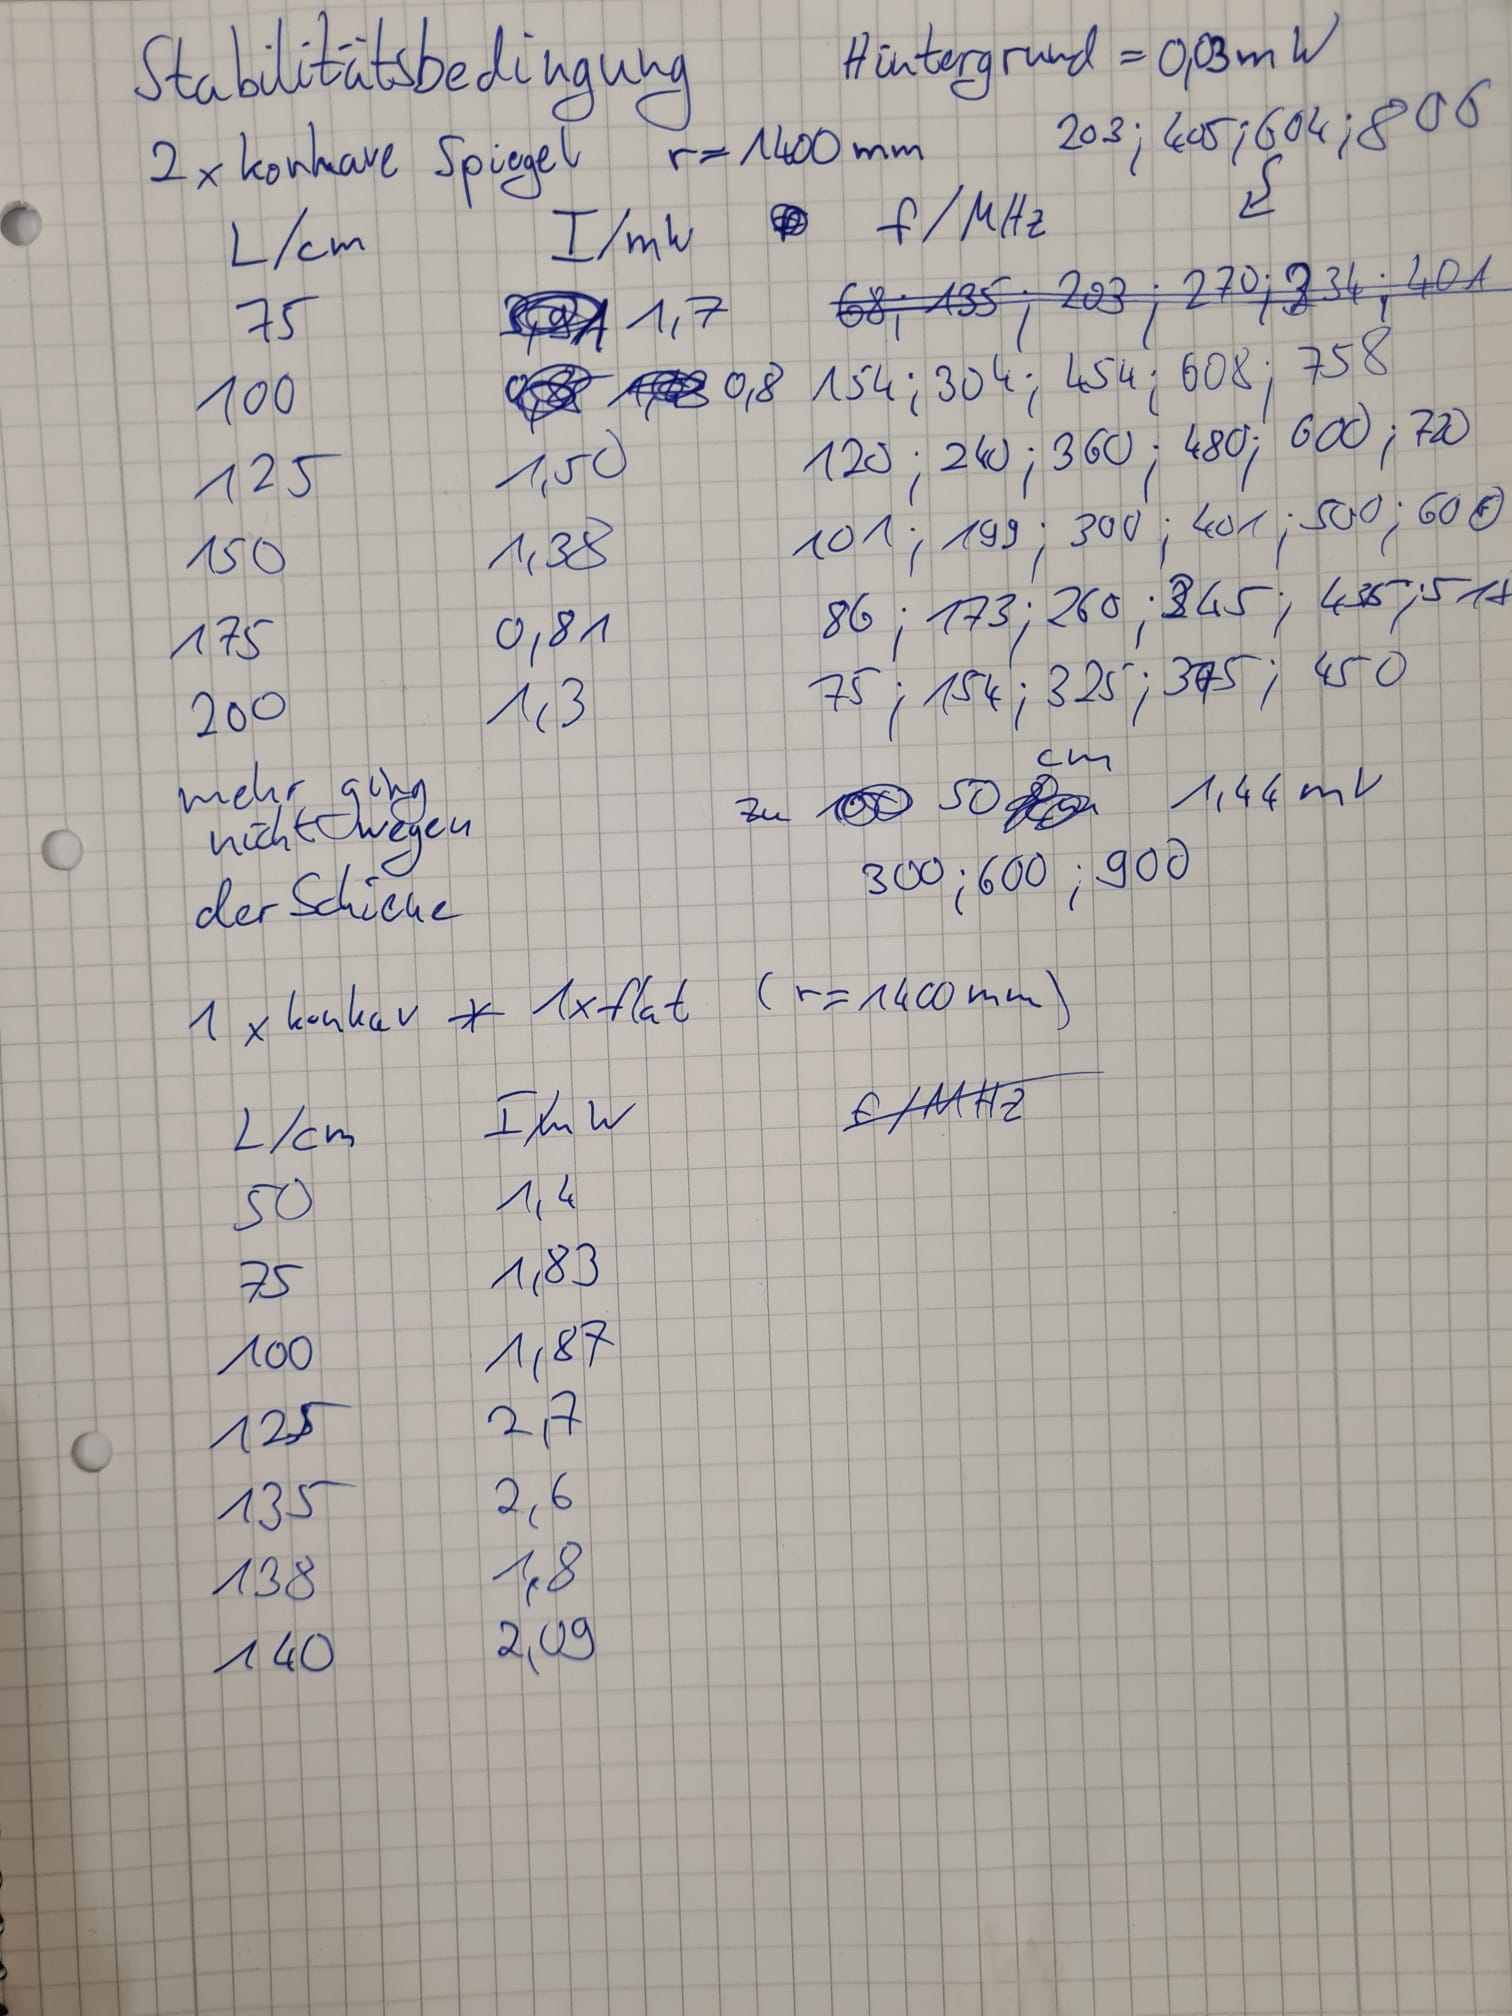
\includegraphics[height=6cm]{content/pics/stabil.jpg}
    \caption{Messwerte der Stabilitätsmessung und Frequenzbreite.}
\end{figure}

\begin{figure}
    \centering
    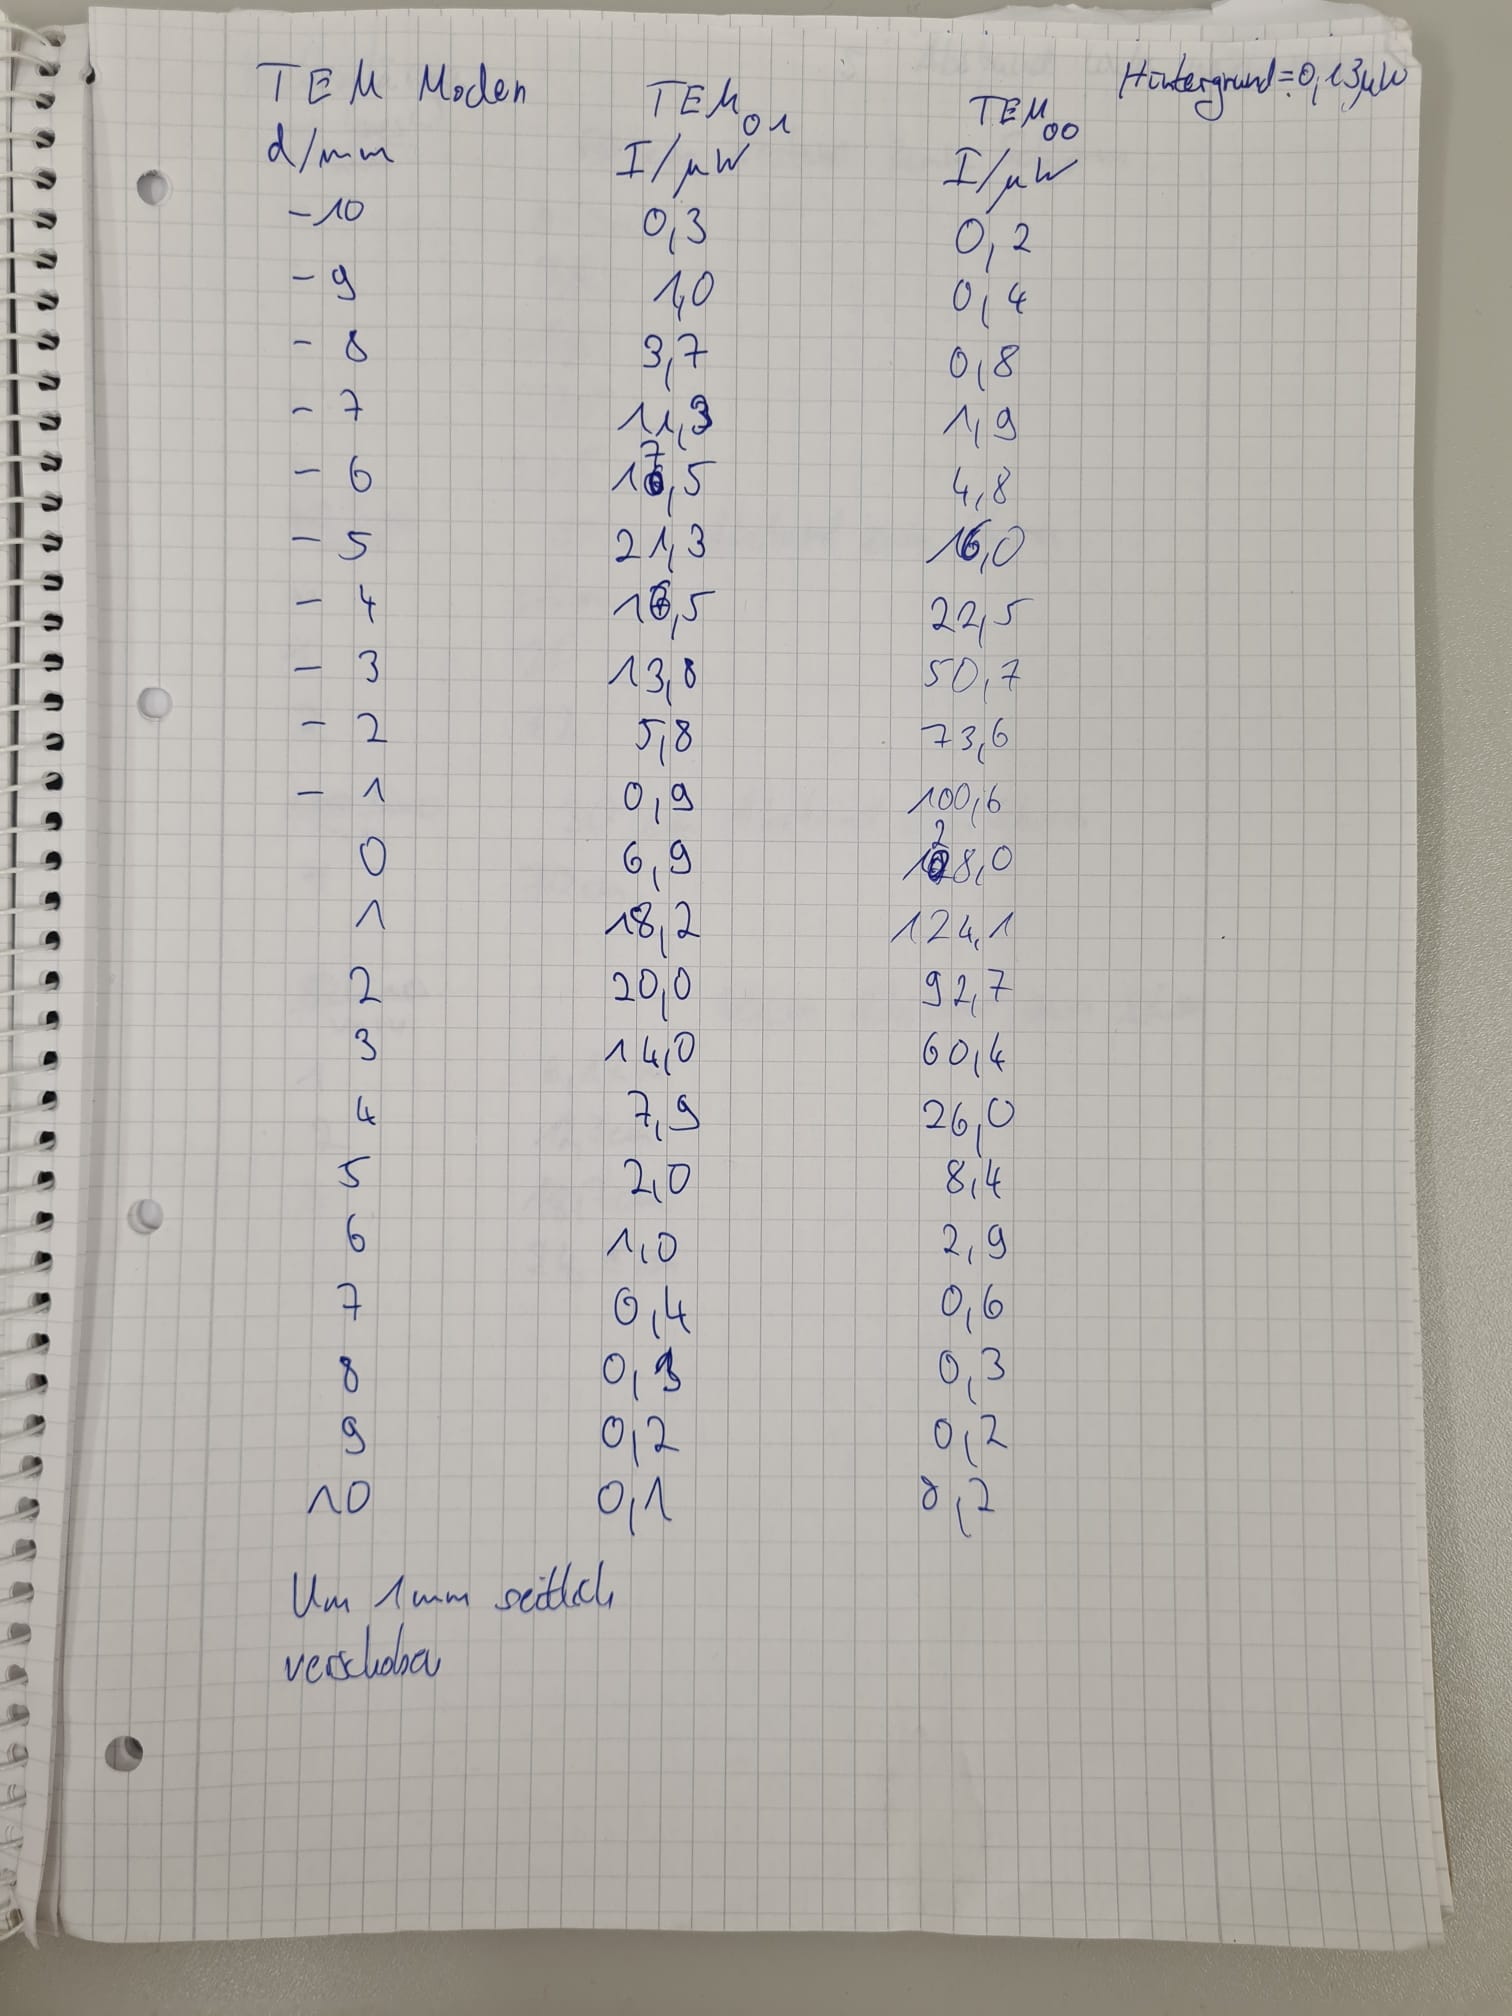
\includegraphics[height=6cm]{content/pics/TEM.jpg}
    \caption{Messwerte der TEM-Moden Messung.}
\end{figure}

\begin{figure}
    \centering
    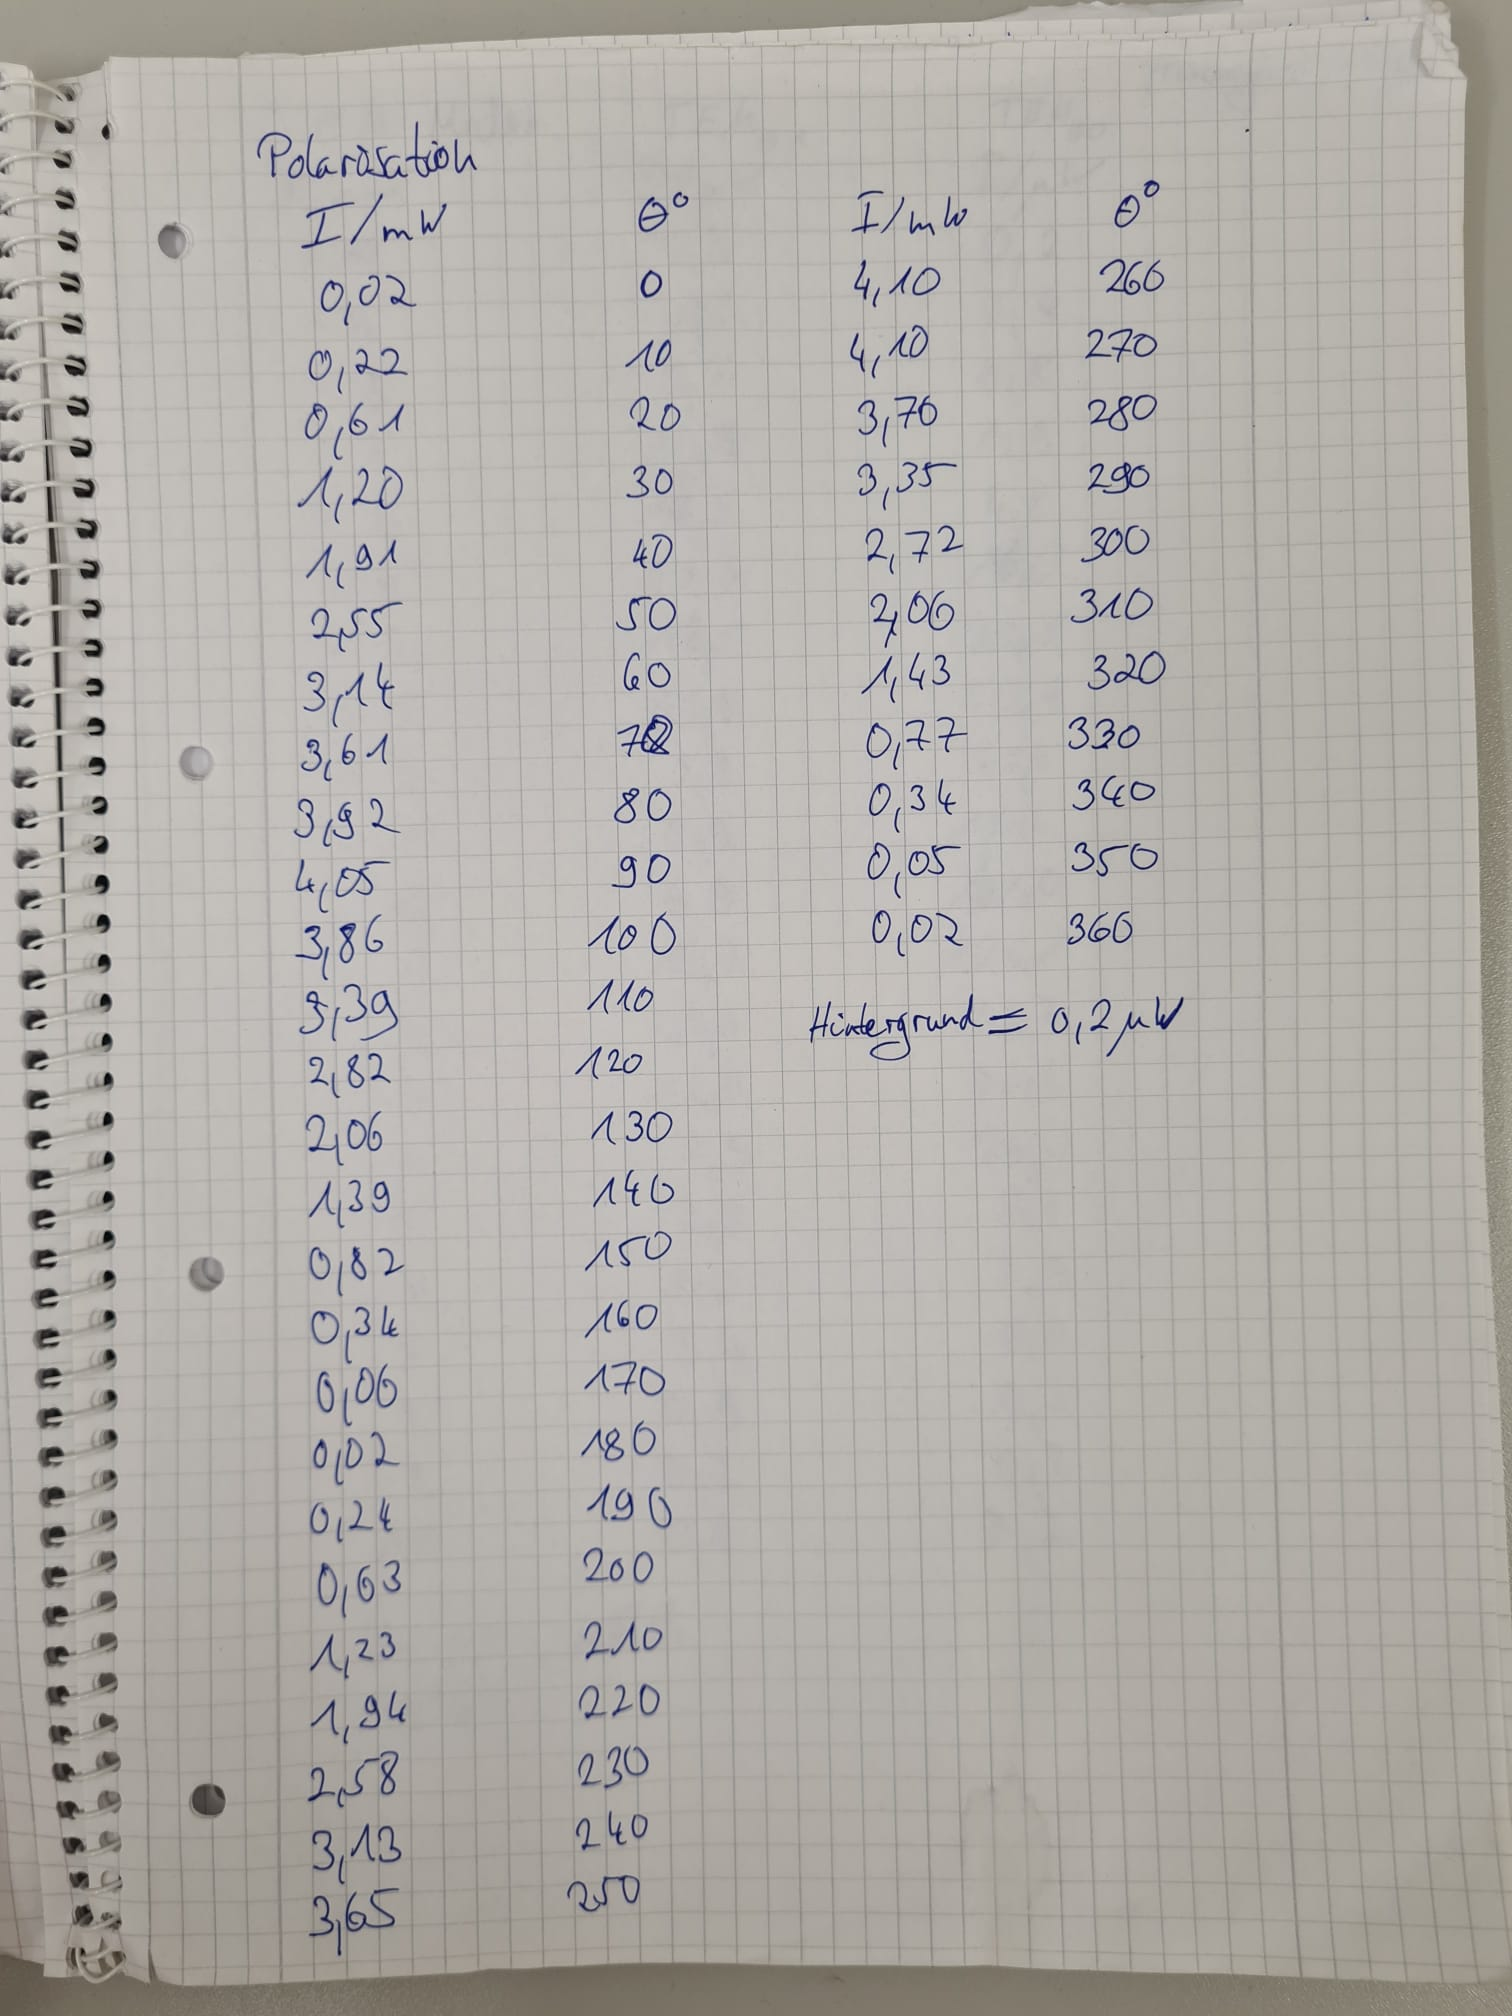
\includegraphics[height=6cm]{content/pics/polarisation.jpg}
    \caption{Messwerte der Polarisationsmessung.}
\end{figure}

\begin{figure}
    \centering
    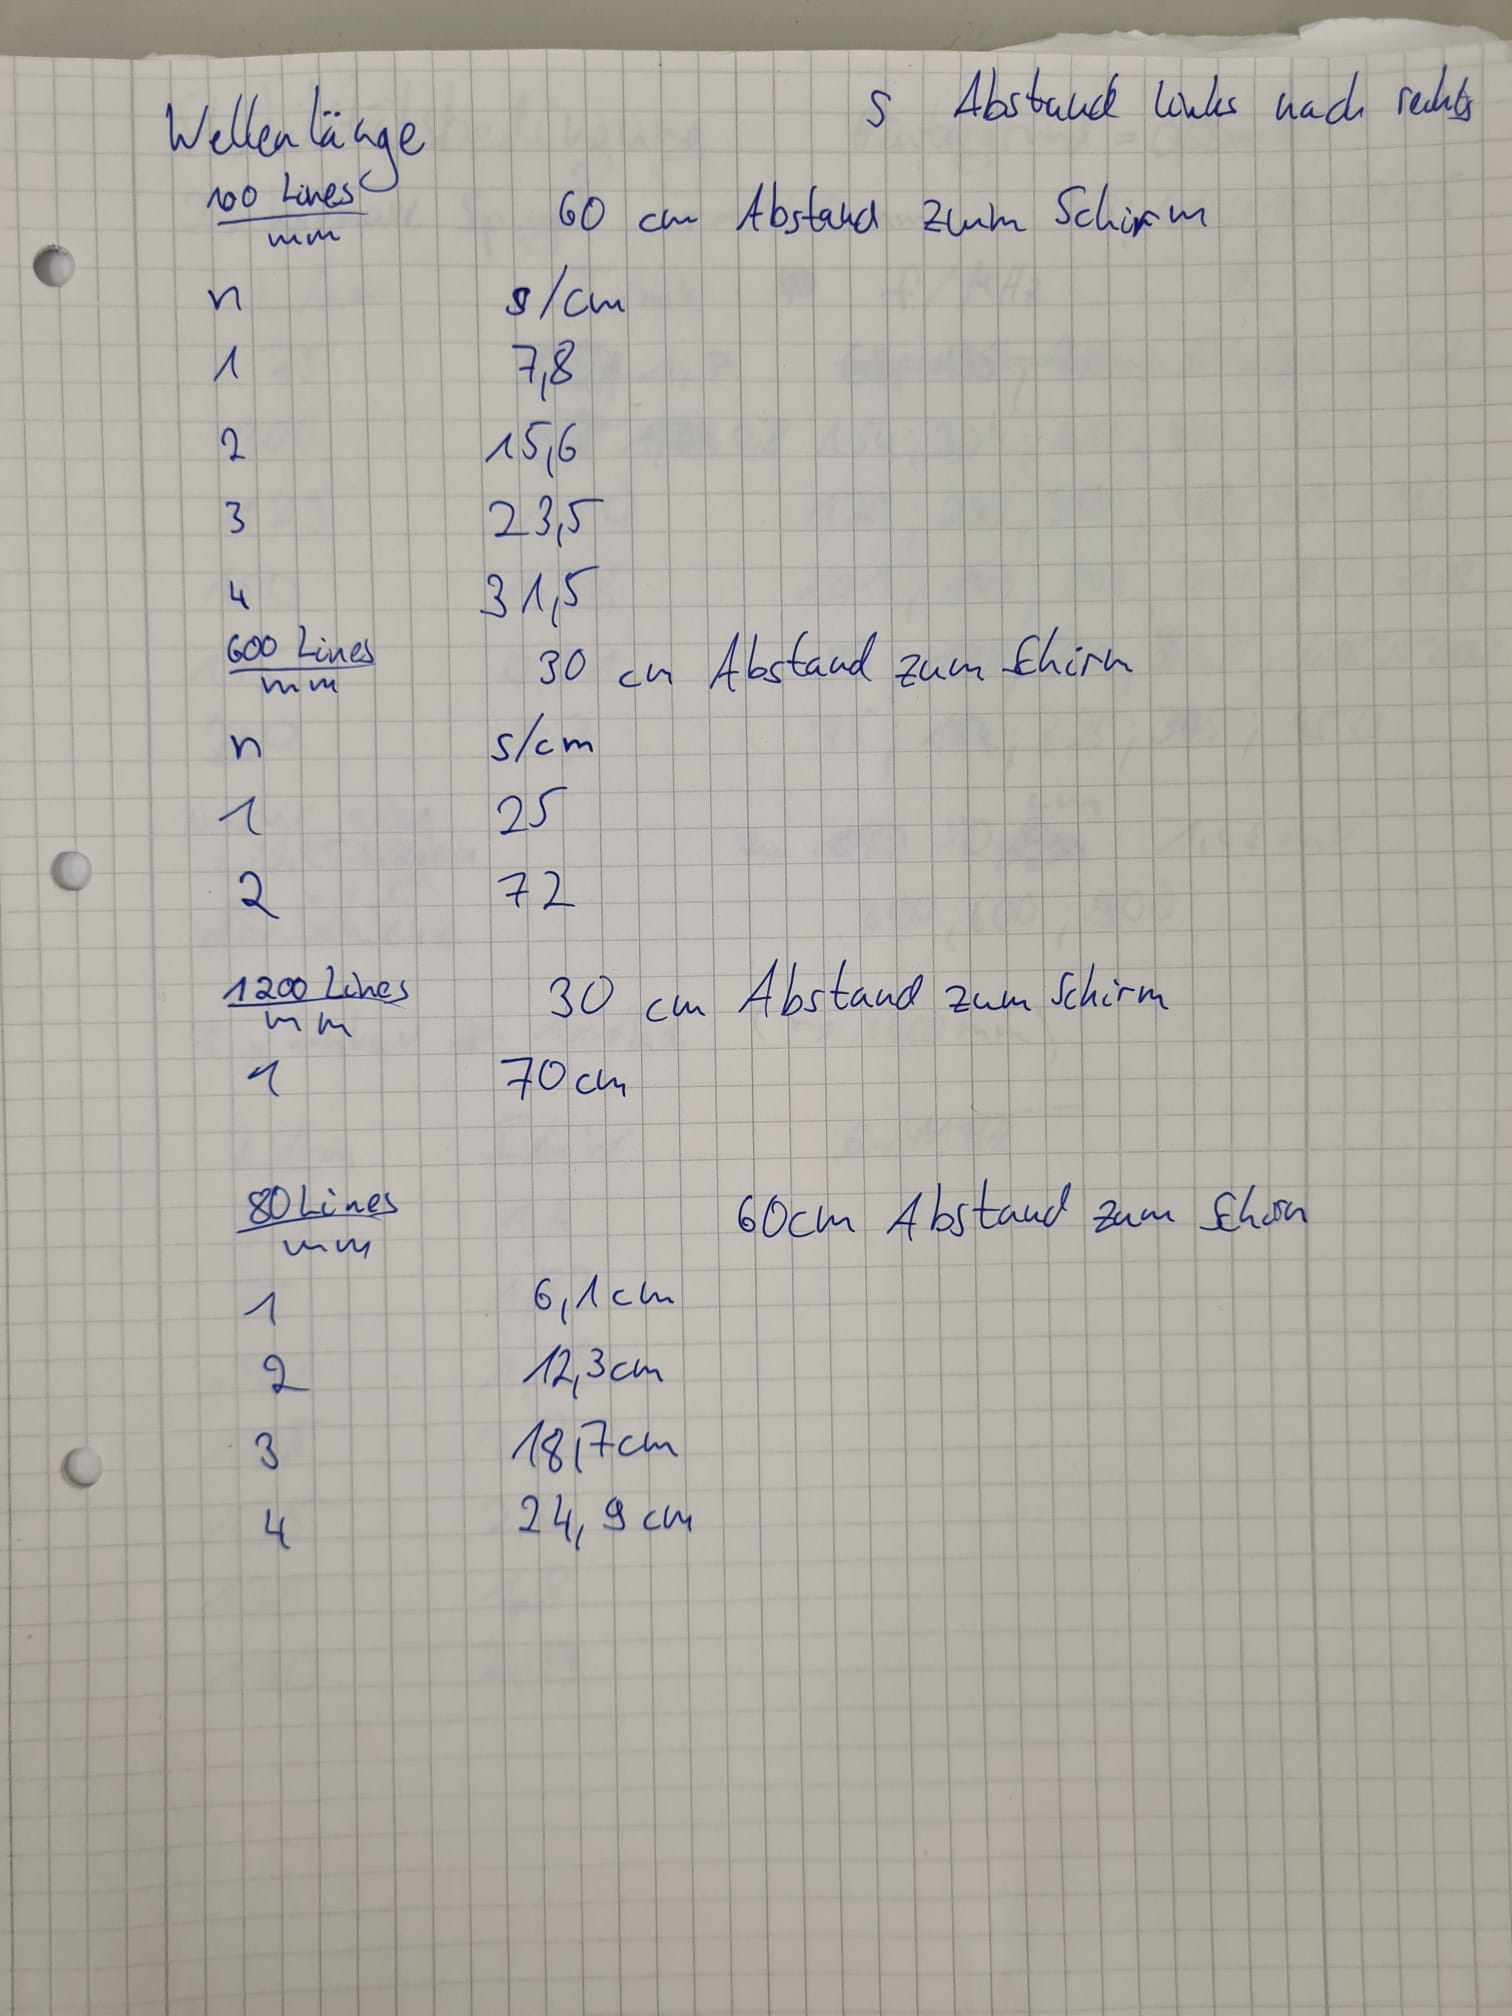
\includegraphics[height=6cm]{content/pics/wellenlaenge.jpg}
    \caption{Messwerte der Wellenlängen Messung.}
\end{figure}